\documentclass[a4paper,11pt]{article}
\usepackage[czech]{babel}
\usepackage[utf8]{inputenc}
\usepackage[pdftex]{graphicx}
\author{Ondřej Pilát}
\title{Napájecí deska pro přestavbu platformy MOB pro použití s RaspberryPi}
\begin{document}
\maketitle
\newpage
\tableofcontents
\newpage
\section{Napájecí deska}
Slouží pro propojení napájení jednotlivých modulů na platformě MOB s 12V bateriemi. Vstupní napětí 12V z baterií, přes proudovou pojistku, je rozděleno na dvě větve 12V a 5V. Převod na 5V je řešen pomocí spínaného zdroje RECOM R-785.0.1.0 s maximálním povoleným proudem 1A. 

Napájecí deska má ochranu proti pod vybití baterií, která odpojí baterie od napájecích větví modulů v případě poklesu napětí baterií pod 10.7V. 

\subsection{Specifikace}

Ochrana proti pod vybití baterií je tvořena dvěma tranzistory, tlačítkem a zenerovou diodou 10V. Při připojení napájení k obvodu je obvod stále otevřen. Až stisknutím tlačítka jsou otevřeny oba tranzistory což vede k uzavření obvodu. Po uvolnění tlačítka jsou tranzistory udržovány v otevřeném stavu přes zenerovou diodu pokud je napětí v obvodu větší než 10.7V. Pokud napětí klesne pod tuto hranici zenerova dioda se uzavře. S ní i tranzistory a celý obvod se otevře.

Ochranný obvod a následně napájecí větve jsou připojeny k bateriím a svorkovnici pro napájení přes ochranou pojistku proti zkratu.
\\
\\
Parametry desky:
\begin{itemize}
	\item 2x svorkovnice pro připojení 12V baterie
	\item 1x svorkovnice pro připojení napájení 12V baterií
	\item 1x svorkovnice pro hlavní vypínač
	\item 1x svorkovnice pro tlačítko připojující napájecí větve s ochranou před pod vybitím baterií
	\item 1x 12V napájecí větev
		\begin{itemize}
			\item 2x dvojité svorkovnice pro připojení 12V modulu s vypínačem
		\end{itemize}
	\item 1x 5V napájecí větev řešená pomocí spínaného zdroje RECOM R-785.0.1.0 s maximálním odběrem 1A
		\begin{itemize}
			\item 4x svorkovnice pro přímé připojení napájení 5V modulů
		\end{itemize}
	\item Velikost desky 3.3 x 1.8 palců
	\item Rozteč děr je 3 x 1.5 palců a průměr díry je 3.2mm.
\end{itemize}

\newpage
\subsection{Struktura a zapojení desky}

\begin{figure}[htbp]
	\centering
		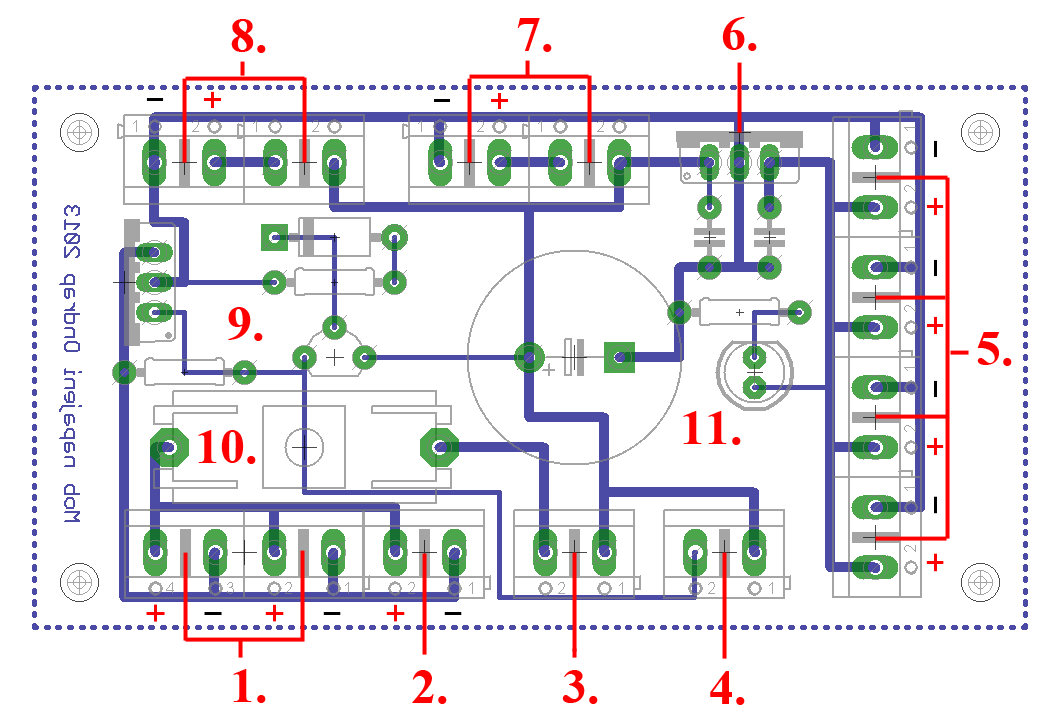
\includegraphics{napajeniMobDeskaOznacena.png}
	\label{fig:napajeniMobDeskaOznacena}
	\caption{Napájecí deska s označením důležitých částí}
\end{figure}

\begin{enumerate}
	\item svorkovnice pro připojení 12V baterií. 
	\item svorkovnice pro připojení napájecího konektoru k bateriím.
	\item svorkovnice pro připojení hlavního vypínače.
	\item svorkovnice pro připojení tlačítka pro sepnutí ochrany proti pod vybití a zároveň připojení baterií k napájecím větvím.
	\item svorkovnice pro připojení napájení 5V modulů.
	\item spínaný zdroj RECOM R-785.0.1.0 pro převod vstupního napětí 12V na výstupní 5V.
	\item svorkovnice pro zapojení vypínače a napájení 12V modulu.
	\item svorkovnice pro zapojení vypínače a napájení 12V modulu.
	\item součástky ochrany proti pod vybití baterií.
	\item ochranná pojistka proti zkratu oddělující baterie od napájecích větví.
	\item dioda indikující zapnutí napájení modulů.
\end{enumerate}

\newpage
\subsection{Schéma desky}
\begin{figure}[ht]
	\centering
		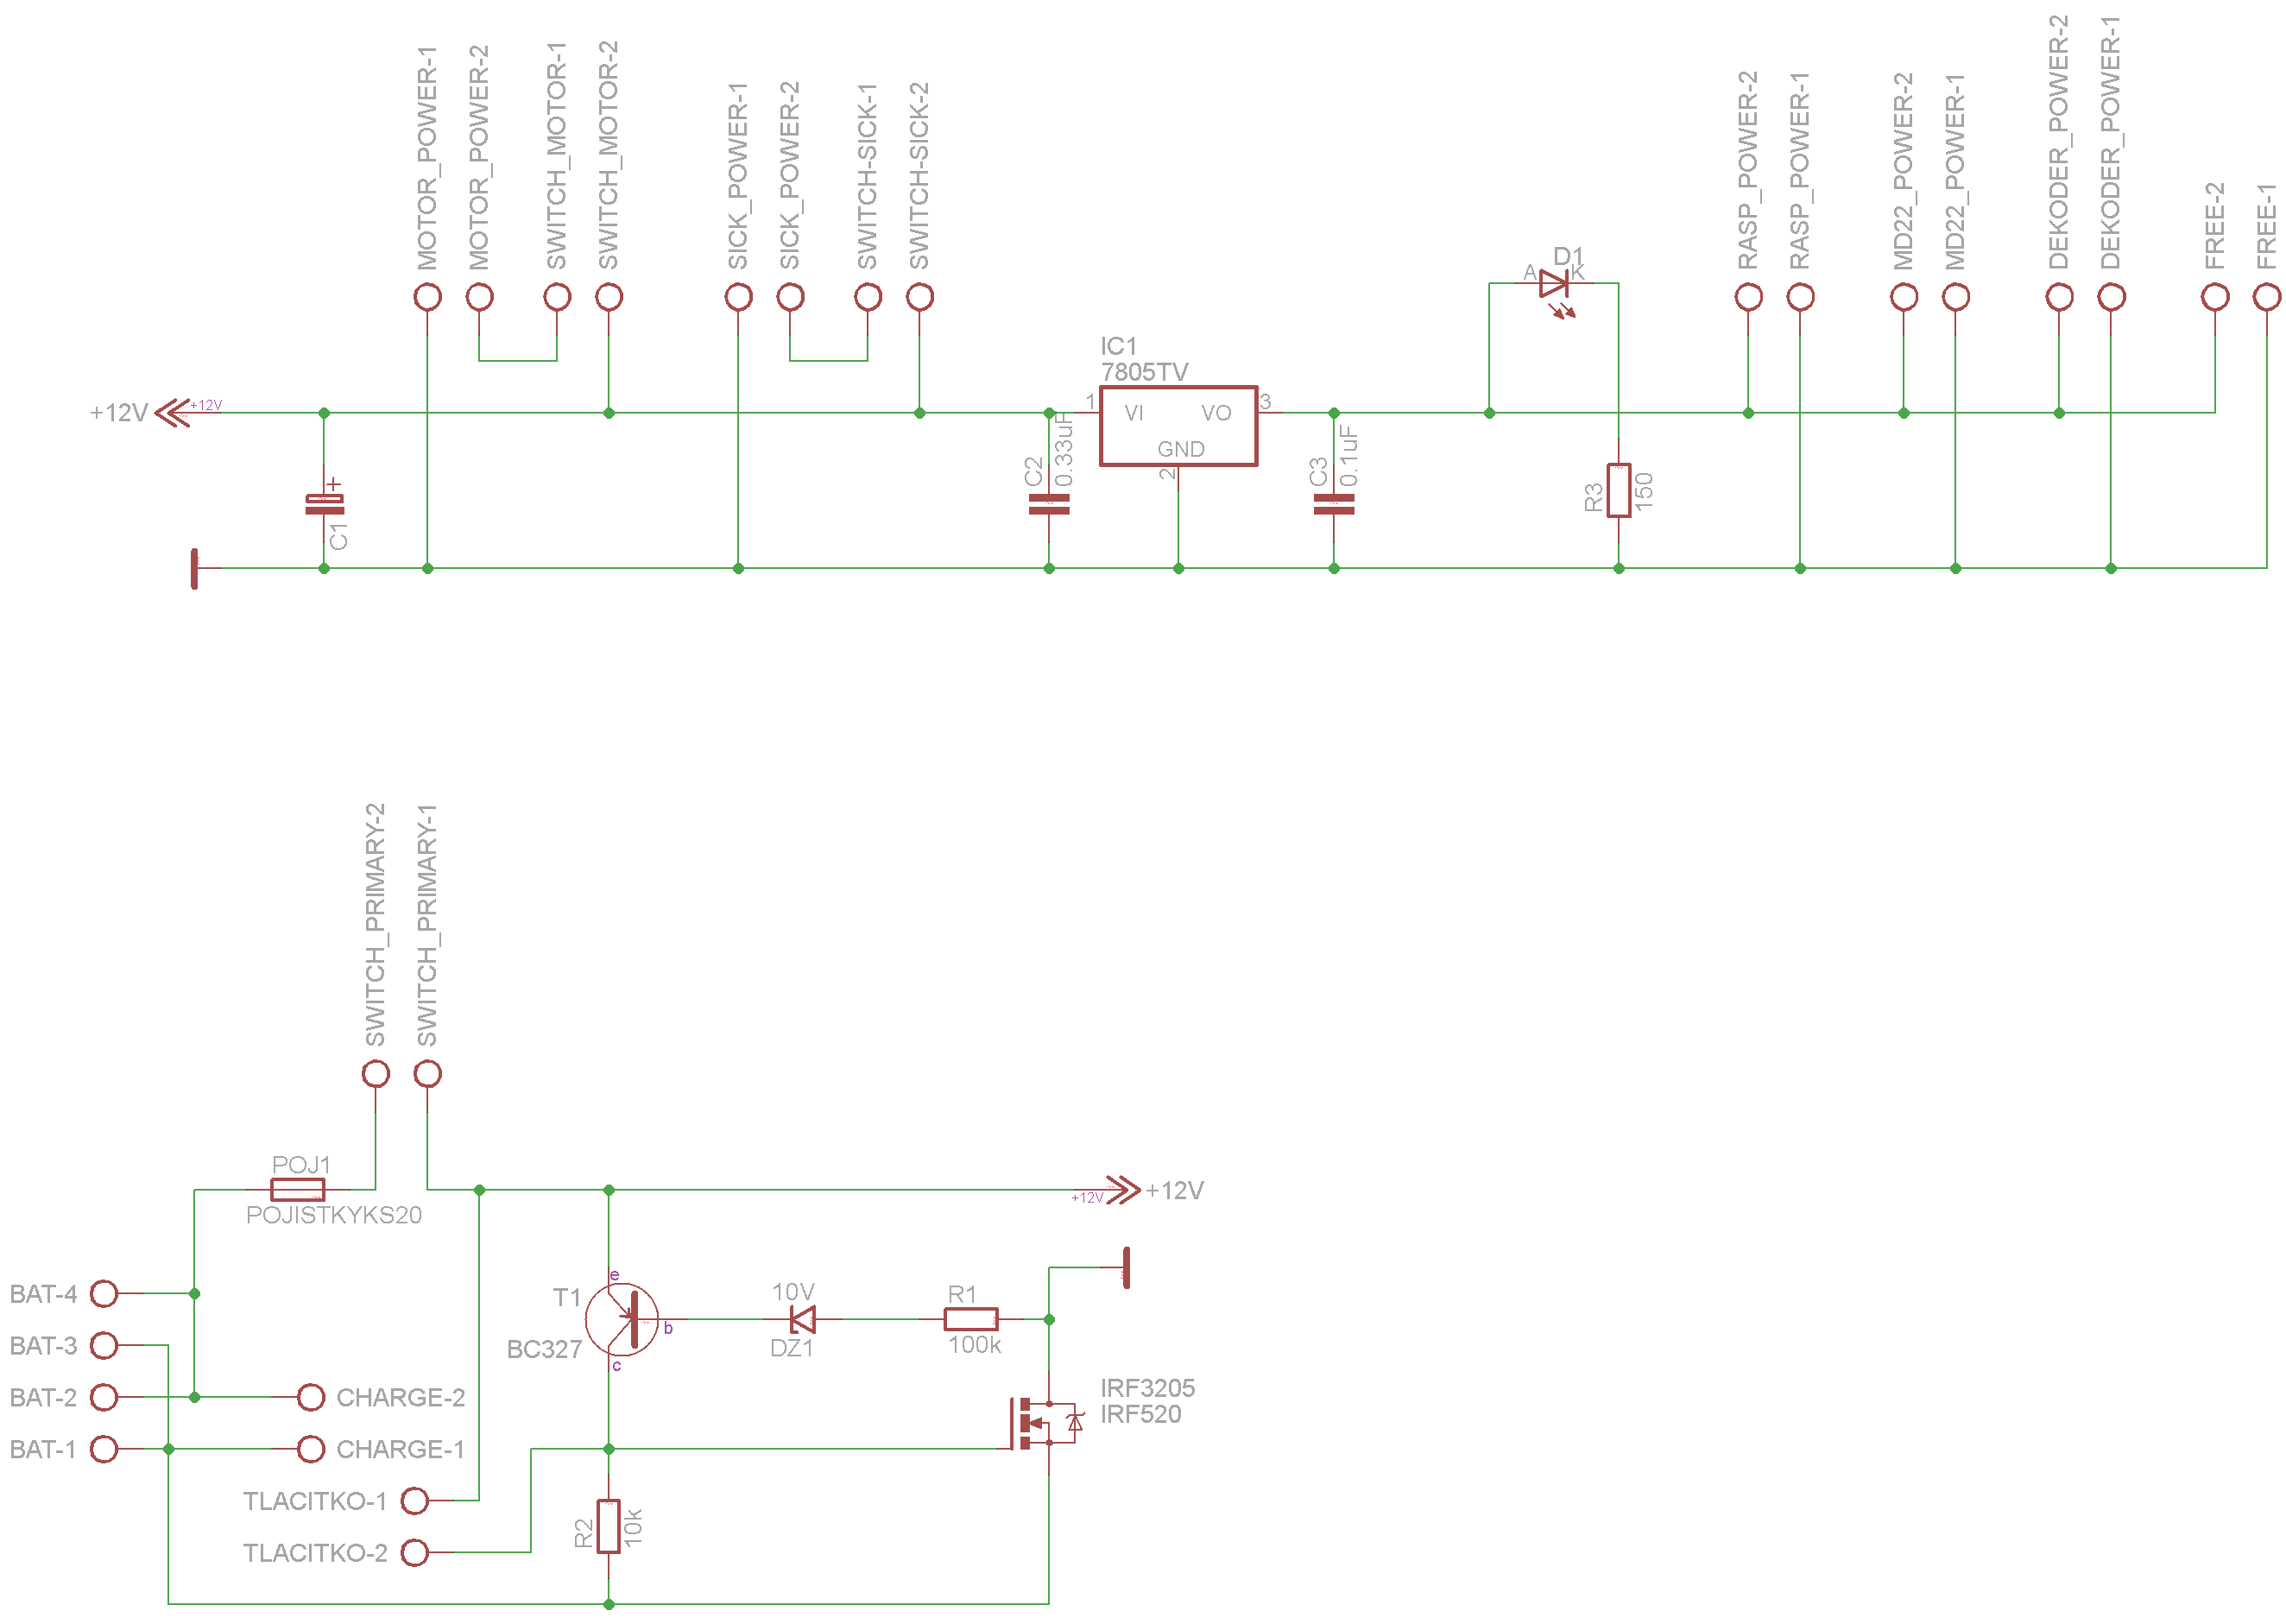
\includegraphics[scale=0.65]{napajeniMobSchema.png}
	\caption{Schéma zapojení napájecí desky}
	\label{fig:napajeniMobSchema}
\end{figure}


\end{document}
